\section{Implementation details}

This section describes implementation details of the proposed solution. 
It highlights key aspects of the core implementation, OpenCL specifics, optimization of particular operations, and high-level optimizations of graph algorithms. It gives an insight into the selected storage formats, algorithms for GPU processing, and chosen third-party instruments for the library foundation.

\subsection{Project structure}

Developed spla library is written using C++17 language and standard library. CMake 3.17 is used as build configuration tool. Ninja library is used to generate platform specific build files. Library supports build on Linux (tested on Ubuntu 20.04), Windows (tested on 10) and macOS (tested on Catalina). Git used as version control system. The source code of the project is hosted on a GitHub page. Library is compiled into shared executable object with respect to the target platform naming convention and object extension.\\

Project directory has the following structure.\\

\begin{itemize}[noitemsep,topsep=0pt,parsep=0pt,partopsep=0pt]
    \item {\fontspec{Symbola}\symbol{"1F5C0}} \textit{include}. Public library interface files in \textit{.hpp} and \textit{.h} format. 
    \item {\fontspec{Symbola}\symbol{"1F5C0}} \textit{src}. Source files, compiled into shared executable object.
    \item {\fontspec{Symbola}\symbol{"1F5C0}} \textit{deps}. Third-party project dependencies stored as a source code.
    \item {\fontspec{Symbola}\symbol{"1F5C0}} \textit{tests}. Directory with unit tests files for Google Tests.
    \item {\fontspec{Symbola}\symbol{"1F5C0}} \textit{examples}. Example applications for graph algorithms.
    \item {\fontspec{Symbola}\symbol{"1F5C0}} \textit{python}. Source code for a python package for spla library.
    \item {\fontspec{Symbola}\symbol{"1F5CE}} \textit{CMakeLists.txt}. Root cmake file of the project.
    \item {\fontspec{Symbola}\symbol{"1F5CE}} \textit{build.py}. Python script to build library artifacts.
    \item {\fontspec{Symbola}\symbol{"1F5CE}} \textit{generate.py}. Python script to generate \textit{.hpp} from \textit{.cl} files.
    \item {\fontspec{Symbola}\symbol{"1F5CE}} \textit{run\_tests.py}. Python script to run unit tests.
    \item {\fontspec{Symbola}\symbol{"1F5CE}} \textit{bump\_version.py}. Python script to upgrade package version.
\end{itemize}

\subsection{Compile-time dependencies}

This section briefly covers third-party libraries and projects, utilized by the spla library.\\

\textbf{Khronos OpenCL headers}. C-compatible OpenCL header files library developed and maintained by the Khronos Consortium. Since the OpenCL is an public API declared as a standard, its support is optional for operating systems and programming environments. In order to access OpenCL functions the respective header files with OpenCL functions declarations, signatures, constants, defines and other symbols must be manually used by a project. An alternative is to install this headers to a computer manually. But this step is error prone and less flexible.\\

\textbf{Khronos OpenCL hpp headers}. C++-compatible OpenCL header files library developed and maintained by the Khronos Consortium. Since the spla project is written using modern C++ standard, safe C++ bindings for an OpenCL code must be used. 

OpenCL C++ bindings provide a memory and exceptions safe, object-oriented API, which relies on a standard containers and data structures. It allows to automate and simplify objects lifetime management. \\

\textbf{Khronos OpenCL ICD loader}. OpenCL installable client driver (ICD) library developed and maintained by the Khronos Consortium. It provides a mechanism to allow developers to build applications against an ICD loader rather than linking their applications against a specific OpenCL implementation. 

The ICD loader is responsible for: exporting OpenCL API entry points, enumerating OpenCL implementations, forwarding OpenCL API calls to the correct implementation.

The ICD mechanism is required in order to load dynamically particular OpenCL implementation at runtime. The motivation for that is the vast variety of different OpenCL implementations. Each implementation can be shipped with a GPU driver. The system can have a number of different GPUs with distinct drivers and vendors. Thus, it is not possible to know a target implementation a priory.

The ICD loader is bundled inside the spla dynamic library during build process. Loader is used on a library startup. It quires available OpenCL drivers in the system. Then it selects one to use in the application. The selection is based on a user parameters. Then it loads OpenCL symbols through shared library mechanism and initializes global OpenCL state.\\

\textbf{GTest}. GTest is an open source unit-testing library for C++ projects. This library is developed and maintained by a Google company. The library provides flexible macro system for declaring unit tests and assertions. This library is used extensively for testing a spla functionality. Project units testes with gtest are stored in a \textit{tests} directory.\\

\textbf{Cxxopts}. Cxxopts is an open-source command-line arguments parsing library for C++ projects. This library automates processing of executable arguments, passed in a classic \textit{argc \& argv} fashion. Library is used a an auxilary tool for example applications, built using library API. Example applications used for a benchmarking of the library performance.\\

\subsection{Development automation}

The library source code is hosted on a GitHub platform. This platform provides a convenient \textit{actions} mechanism, also called \textit{workflows}. It allows to automate the process of a continuous project changes integration and continuous delivery of the project artifacts to potential users. The GitHub repository is configure with the following list of scripts for automation.

\begin{itemize}
    \item \textbf{build}. The build action, which compiles the source code of the library, executable examples and test for three target platform: Windows 10, Ubuntu (20.04) and macOS (for x64 and arm architectures). The artifacts of a build process are published automatically in a GitHub repository. These artifacts are reused in a later step, when the python package is assembled to be pushed to either test or retail index repository.  
    
    \item \textbf{clang-format}. The formatting script which automatically checks the conformance of the library header and source files. The project uses a clang-format tool to check the code style of the project automatically. Definition of a code style is stored in repository as a configuration file in special format.  
    
    \item \textbf{deploy}. Deployment script is responsible for an automated publishing of a spla python package to the python package index (PyPI) repository. This action assembles a bundle, which stores python sources as well as artifacts for all platforms from \textit{build} action. Action automatically pushes package to the PyPI using credentials, stored in a repository. The action is triggered automatically on commits to special \textit{release} branch. This is supposed to happen on a major and minor library versions' releases. 
    
    \item \textbf{deploy-test}. Deployment script similar to \textit{deploy} action. The difference is that this script pushes package to the Test PyPI repository for testing purposes. The action is triggered automatically on commits to special \textit{pre-release} branch.
    
    \item \textbf{docs-cpp}. Script which assembles C/C++ library documentation using Oxygen format. The documentation is represented by a set of html pages. These pages are deployed automatically to the project website page. 
    
    \item \textbf{docs-pythos}. Script which assembles python package documentation using python docs library. The documentation is represented by a set of html pages. These pages are deployed automatically to the project website page. 
\end{itemize}

\subsection{Library interface}

This section the technical details of the library public interface are covered. Interface includes matrix, vector and scalar containers for a typed data storage, operations for the execution, algebraic functions for operations customization, etc.\\

\textbf{Containers}. Library provides \textit{vector}, \textit{matrix} and \textit{scalar} data containers. Each container can be parameterised with a type of stored values. The actual storage mechanism is automated and is hidden from a user. Matrix and vector containers can store data in multiple formats at the same time. In order to access them, the library provides opaque interface, which allows to incrementally build containers, query elements, inspect its properties an state. List of supported operations to access containers is shown in a table~\ref{tab:containers}.\\

\begin{table}[tbp]
\caption{A list of the supported operations to access vector and matrix containers.}
\begin{center}
    \rowcolors{2}{black!2}{black!10}
    \begin{tabular}{|l|l|l|}
    \hline
    \textbf{Method} & \textbf{Description} \\ \hline
    \hline
    \textit{Matrix} & Matrix constructor from type T and dimensions\\ \hline
    \textit{Vector} & Vector constructor from type T and dimension\\ \hline
    \hline
    \textit{clear} & Empty vector or matrix\\ \hline
    \hline
    \textit{get\_nrows} & Query number of rows for a matrix or vector\\ \hline
    \textit{get\_ncols} & Query number of columns for a matrix or vector\\ \hline
    \textit{get\_type} & Query the type T of elements \\ \hline
    \hline
    \textit{set\_<T>} & Set element of type T at index $\langle i,j\rangle$\\ \hline
    \textit{get\_<T>} & Get element of type T at index $\langle i,j\rangle$\\ \hline
    \end{tabular}
    \label{tab:containers}
\end{center}
\end{table}

\textbf{Operations}. An expression for the execution is constructed as a schedule object using library API. The primitive unit of the schedule is a single task. Task represents an operation over matrices, vectors and scalars. Library provides a number of common and widely used operations for evaluation. List of supported operations provided in the table~\ref{tab:operations}.\\

\begin{table}[tbp]
\caption{A list of the spla mathematical operations for computations.}
\begin{center}
    \rowcolors{2}{black!2}{black!10}
    \scalebox{0.8}{
    \begin{tabular}{|l|l|l|}
    \hline
    \textbf{Operation}     & \textbf{Math equivalent}               & \textbf{Description}           \\ \hline 
    \hline
    \textit{masked mxmT}   & $R_{i,j} = (AB^T)_{i,j}, \forall i,j: f(M_{i,j})$ & Masked matrix-matrix transposed product\\ \hline
    \hline
    \textit{masked vxm}    & $r_i = (vM)_i, \forall i: f(m_i)$   & Masked vector-matrix product   \\ \hline
    \textit{masked mxv}    & $r_i = (Mv)_i, \forall i: f(m_i)$   & Masked matrix-vector product   \\ \hline 
    \hline
    \textit{reduce by row} & $r_i = \Sigma M_{i,j}$              & Matrix reduce by row to column vector \\ \hline
    \textit{ewise add}     & $r_i = v_i + u_i$                   & Vector element-wise addition   \\ \hline    
    \textit{masked assign} & $r_i = s, \forall i: f(m_i)$        & Masked vector scalar assignment\\ \hline 
    \textit{map}           & $r_i = g(v_i)$                      & Vector map to vector using unary function \\ \hline
    \hline
    \textit{reduce}        & $s = \Sigma M_{i,j}$                   & Matrix reduce to scalar        \\ \hline
    \textit{reduce}        & $s = \Sigma v_i$                       & Vector reduce to scalar        \\ \hline
    \textit{select count}  & $s = |\{v_i: f(v_i)\}|$                & Vector select count            \\ \hline
    \end{tabular}
    }
    \label{tab:operations}
\end{center}
\end{table}

\textbf{Element-wise functions}. The core feature of the library is the ability to parameterise math operations mentioned above with arbitrary algebraic element-wise binary and unary functions. The list of build-in functions, which supported for both CPU and GPU computations, is depicted in the table~\ref{tab:ewise}. The operations can be used for any of build type such int, uint and float values. The only exception is bit-wise operations, which can be applied only to integral types.\\

\begin{table}[tbp]
\caption{A list of the spla element-wise mathematical functions to parameterise operations.}
\begin{center}
    \rowcolors{2}{black!2}{black!10}
    \scalebox{0.8}{
    \begin{tabular}{|l|l|l|l|}
    \hline
    \textbf{Function} & \textbf{Equivalent} & \textbf{Type} & \textbf{Description} \\ \hline
    \hline
    \textit{plus}   & $r = a + b$ & function & Sum of two elements \\ \hline
    \textit{minus}  & $r = a - b$ & function & Difference of two elements \\ \hline
    \textit{mult}   & $r = a * b$ & function & Product of two elements \\ \hline
    \textit{div}    & $r = a / b$ & function & Division of two elements \\ \hline
    \hline
    \textit{min}    & $r = min(a, b)$ & function & Minimum value \\ \hline
    \textit{max}    & $r = max(a, b)$ & function & Maximum value \\ \hline
    \hline
    \textit{first}  & $r = a$ & function & First argument of function \\ \hline
    \textit{second} & $r = b$ & function & Second argument of function \\ \hline
    \textit{one}    & $r = 1$ & function & Identity element \\ \hline
    \hline
    \textit{and}    & $r = a \land b$  & function & Bit-wise product \\ \hline
    \textit{or}     & $r = a \lor b$   & function & Bit-wise sum\\ \hline
    \textit{xor}    & $r = a \oplus b$ & function  & Bit-wise exclusive sum \\ \hline
    \hline
    \textit{eqzero} & $a == 0$  & predicate & Check equals zero \\ \hline
    \textit{nqzero} & $a\neq 0$ & predicate & Check not-equals zero \\ \hline
    \textit{gtzero} & $a > 0$   & predicate & Greater than zero \\ \hline
    \textit{ltzero} & $a < 0$   & predicate & Less than zero \\ \hline
    \textit{geero}  & $a >= 0$  & predicate & Greater equals zero \\ \hline
    \textit{lezero} & $a <= 0$  & predicate & Less equals zero \\ \hline
    \end{tabular}
    }
    \label{tab:ewise}
\end{center}
\end{table}

\textbf{Signatures}. Library heavily relies on a built-in mechanism of automated reference counting of objects. Each object has an atomic counter, which tracks number or references. When the counter reaches the zero, it frees up the object. This mechanism used for safe arguments passing around library and for safe marshaling of objects through C and python APIs.

Library employs explicit operations signatures. All arguments and parameters must passed by the user through operation interface. If operation has variations or provides tweaking, all parameters must be specified.

As an example, consider the signature of the masked matrix-vector product operation in a listing~\ref{alg:spla_op_example}. This is a procedure, which can be loaded from a dynamic or shared library. As the result of an invocation it returns special \textit{Status} enumeration value. Library uses no exceptions. Thus, error codes are employed. It is standard practice for libraries with C-compatible API. 

The procedure takes nine input in lines \textbf{1 -- 9} and one optional output argument in line \textbf{10}. The \textit{r} is a vector where to store result of operation execution. The \textit{mask} is a vector of the same dimension as r, which is used to update only selected entries of the vector r. Matrix \textit{M} and vector \textit{v} are the actual primitives to multiply. Actual algebraic element-wise functions from multiplication and addition are passed as \textit{op\_multiply} and \textit{op\_add}. The predicate to filter result by a mask passed as a \textit{op\_select}. Note, that functions in the library are first-class objects, which can be manipulated as any other library object. The identity element for product evaluation is passed as \textit{init} scalar.

An optional parameter is a Descriptor \textit{desc} object. It has the same usage as in a GraphBLAS standard. Descriptor stores additional parameters, which configure actual execution of the operation, occupation, preferred device, mode, etc. It can be used to optimize the execution of particular operations for edge cases.

Finally, the procedure accepts an optional output argument. It is a pointer to the handle of the schedule task object. If pointer is null, then the procedure executes the operation in an imperative fashion. If this pointer is not null, then the implementation creates a deferred task for the execution, stores reference to this task in provided pointer and returns. In this case, the returned task can be used to construct schedule object, which can be submitted at once as a whole. The scheduling mechanism implemented as previously described in architecture section.

\lstset{style=codelistingstyle}

\begin{algorithm}[tbp]
\floatname{algorithm}{Listing}
\caption{The C++ signature of the spla masked matrix-vector product.}
\label{alg:spla_op_example}
\begin{lstlisting}[language=C++]
SPLA_API Status exec_mxv_masked(/* in  */ ref_ptr<Vector>        r,
                                /* in  */ ref_ptr<Vector>        mask,
                                /* in  */ ref_ptr<Matrix>        M,
                                /* in  */ ref_ptr<Vector>        v,
                                /* in  */ ref_ptr<OpBinary>      op_multiply,
                                /* in  */ ref_ptr<OpBinary>      op_add,
                                /* in  */ ref_ptr<OpSelect>      op_select,
                                /* in  */ ref_ptr<Scalar>        init,
                                /* in  */ ref_ptr<Descriptor>    desc = nullptr,
                                /* out */ ref_ptr<ScheduleTask>* task_hnd = nullptr);
\end{lstlisting}
\end{algorithm}

\subsection{Algorithms registry}

The implemented library uses the concept of a registry to find operations as shown in Fig.\ref{fig:algo_registry}. A call to a particular operation is stored as a command to be executed later by \textit{Dispatcher}. For each command the special lightweight string key is built depending on type of the operation and arguments passed. This key is used as a regex to get the required implementation of the requested operation. The advantages of the proposed approach are listed below.

\begin{itemize}
    \item \textbf{Late binding}. The operation call becomes a command. The processing of such a command can be configured at run time. Changing the acceleration backend can be done without recompilation. Moreover, several backends can be transparently used within a single application.
    
    \item \textbf{Optionality of accelerator}. The acceleration backend is free to support only those operations that require it. Fallback implementations will be used automatically for the rest of the operations.
    
    \item \textbf{Performance tuning}. The key of the command reflects operation type, arguments types, passed user functions types, etc. It can be used for \textit{ad-hoc} optimizations. Custom operation implementation with a verbose key can be also stored in the registry. If several operations match the key, the longest key is used, since it is more specific for a particular operation.
    
    \item \textbf{Scheduling}. The full list of submitted commands for execution can be examined at runtime. This opens up the possibility for the fusion of some operations, sorting, rearrangement, and any other high-level optimizations that require introspection.
\end{itemize}

The structure of keys is depicted in a figure~\ref{fig:algo_key}. The key is effectively a string literal, which is constructed using specialized rules. The prefix of the key is the name of the operation which must be evaluated. As a name for operation actual mathematical name can be used, such as matrix-vector product, matrix-matrix product, etc. 

The name is followed by the name of used functions and their type codes. Mathematical functions must be parameterized by scalar functions. Each function has a name and a set of type codes for each type of the argument. Scalar multiplication and addition functions has three opcodes. Since each function is a binary operator of type $A \times B \xrightarrow{} C$. 

Binary functions are followed by a selection operation. Selection is an unary function with the signature $A \xrightarrow{} bool$. Selection operator is used to filter final results using masking. Typically, we are not interested in a whole result. So the mask is provided. Type of mask values used to parameterize select operation. Selection can be any unary predicate. In most cases, greater than, equals or not equals zero are the most used one.

Finally, the key prefix is appended with a code of a backend  for computations. Different accelerators, including CPU fallback, may be supported for computations. Using accelerator suffix allows to switch between backend at runtime and select the most optimized algorithm. 

It is possible that there is no algorithms for a given key. Thus, the fallback version must be utilized. In order to do that, key prefix may be concatenated with a CPU suffix. All algorithms have a CPU analogues in a registry.

Keys in a form of a string solve two major problems. Firstly, it gives a readable and human understandable representation of an operation. Secondly, it allows to actually segregate an operation with its arguments and particular algorithm instance. Algorithm is an object with its own state and unified interface. It allows to maximize the performance and reuse artifacts, which may appear between algorithm invocations, such as GPU kernels, acceleration structures, etc. 

\begin{figure}
    \centering
    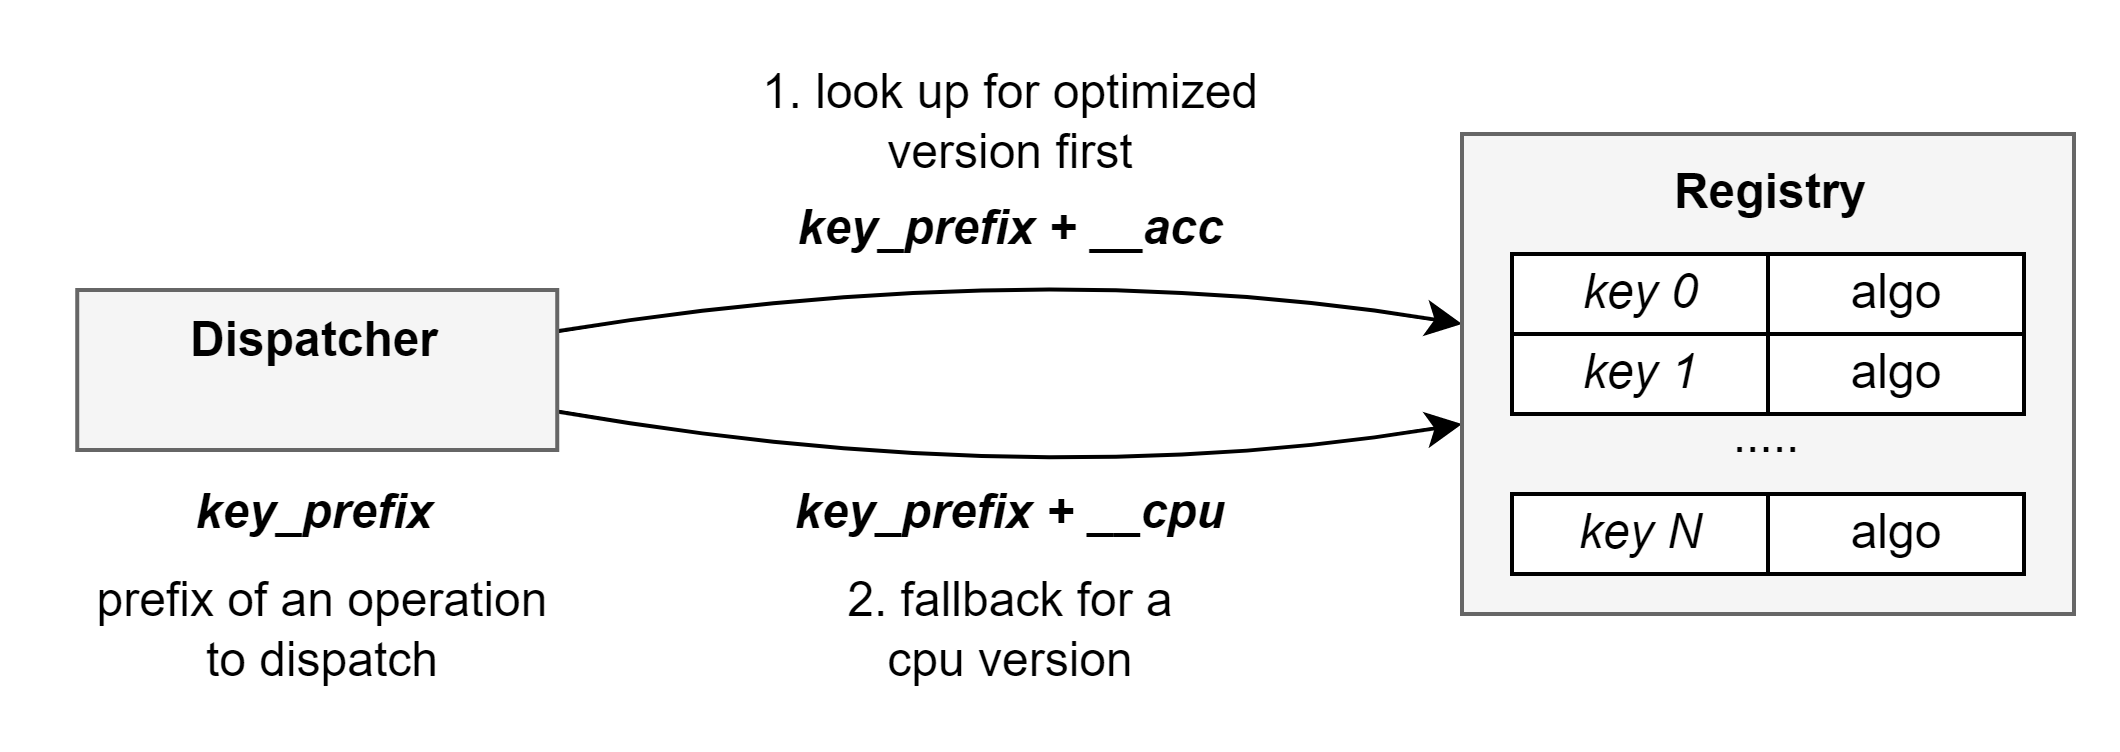
\includegraphics[width=1.0\textwidth]{images/spla_algo_registry.png}
    \caption{Registry of algorithms. Dispatcher looks up for optimized algorithms first. As a fallback it uses cpu suffix to get default algorithm implementation without an acceleration.}
    \label{fig:algo_registry}
\end{figure}

\begin{figure}[]
    \centering
    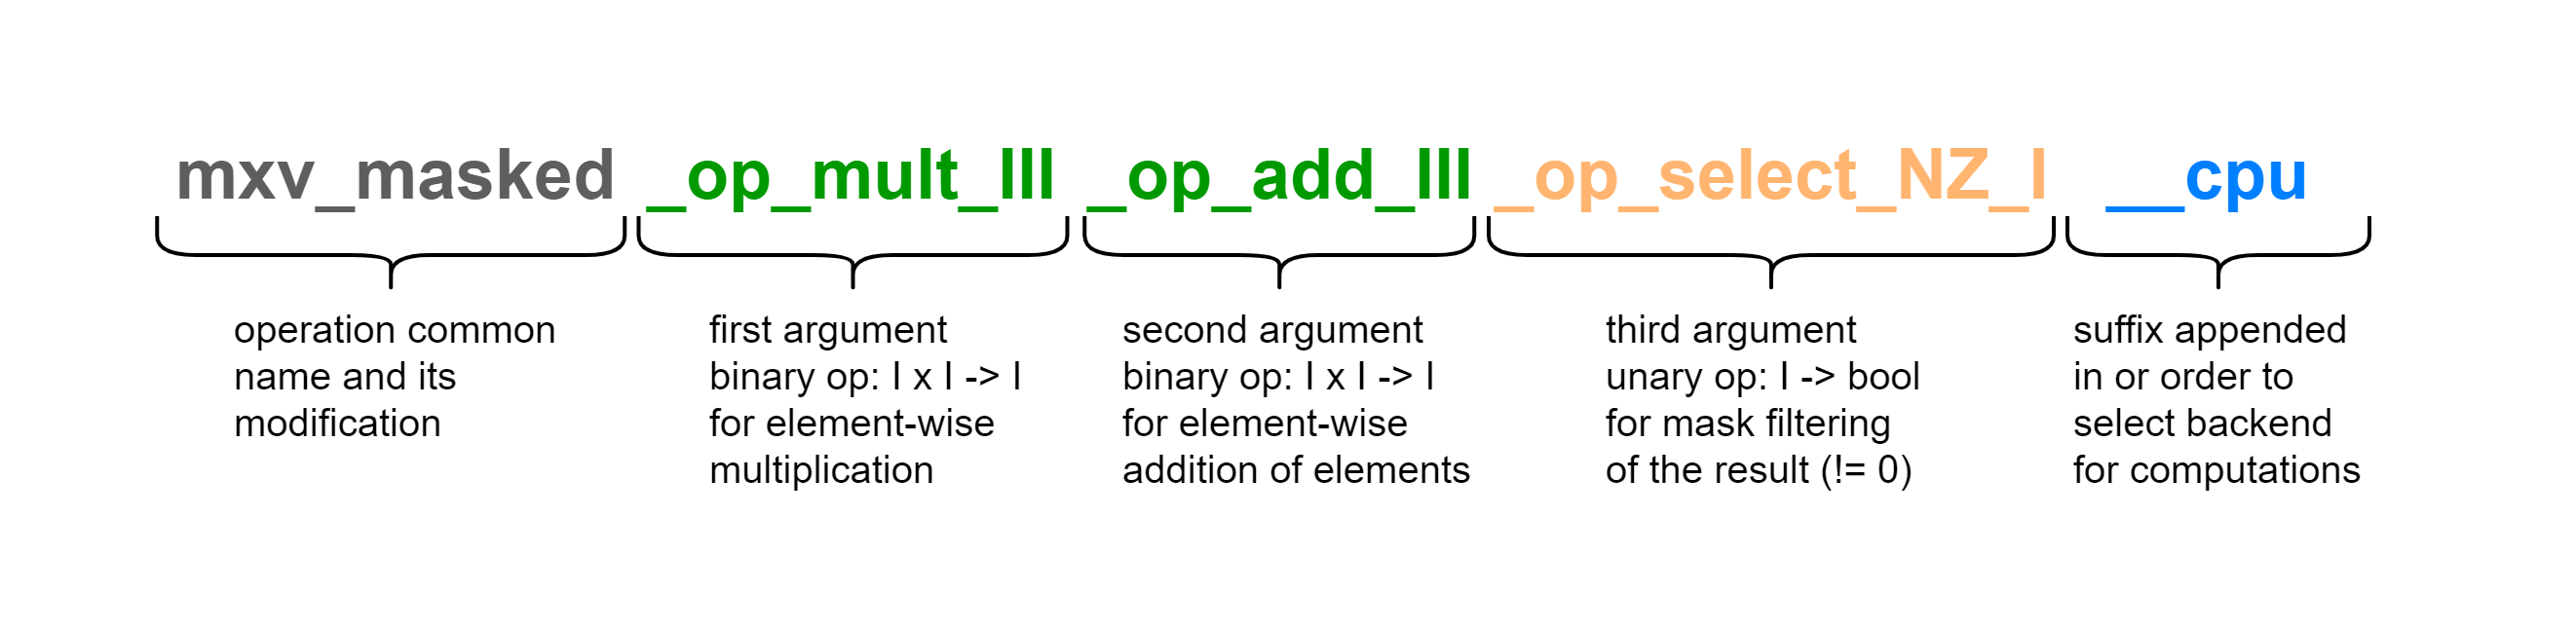
\includegraphics[width=1.0\textwidth]{images/spla_algo_key.png}
    \caption{The structure of an algorithm key. The is a string literal composed from several parts. Prefix shows the algorithm name and its parametrization by operations. The suffix of the key shows which backed or accelerator to use for the evaluation of the algorithm.}
    \label{fig:algo_key}
\end{figure}

\subsection{Storage formats}

The library is implemented following storage schema, introduced and described in a previous section. In this schema each data container, such as a matrix or vector has a number of decorations or formats, which can be simultaneously assigned to the container. It introduces duplication. However, it gives the flexibility for the choice of target device and particular implementation algorithm for the execution.

The same container can have a number of formats allocated at the same time. The storage manager automatically controls the validity of the data. This mechanism allows to cache the same data in both RAM and VRAM memory. Since the RAM in most cases has a order of magnitude larger size, the duplication is negligible.

The vector storage container supports following formats.

\begin{itemize}
    \item \textbf{CPU dictionary of keys (DoK)}. The format of the vector, where non-zero entries stored as a dictionary. Storage space is proportional to a number of values. It gives fast query and insertion operations at cost of inefficient memory layout. This format is used for incremental builds of container on a CPU side.
   
    \item \textbf{CPU list of coordinates (COO).} This format used for sparse vector representation. Data in this format stored as a list of indices and as a list of values. Memory space proportional to the number of non-zero entries. Used to prepare data for GPU source \& target transfer.
   
    \item \textbf{CPU dense vector.} This format used for a dense vector representation. Data in this format stored as a large array of values with the same size as vector dimension. Memory space proportional to the vector dimension. Memory consumption can be excessive on vectors with over 1M elements. Used to prepare data for GPU source \& target transfer.
    
    \item \textbf{OpenCL list of coordinates (COO)}. It is GPU representation of a COO format using OpenCL API. Used for sparse vector manipulation on GPU side. 
    
    \item \textbf{OpenCL dense vector}. It is GPU representation of a COO format using OpenCL API. Used for a dense vector manipulation on GPU side.
\end{itemize}

The matrix storage container supports following formats.

\begin{itemize}
    \item \textbf{CPU dictionary of keys (Dok)}. This format is used for an incremental matrix building on a CPU side as it is done for a vector. The memory space used by this format is proportional to the number of non-zero entries. This format provides fast query and insertion operations at cost of inefficient memory layout.
    
    \item \textbf{CPU compressed sparse row (CSR)}. Compressed sparse row is one of the most common formats for a sparse matrix representation. The data is stored in a form of three arrays: rows offsets, column indices and column values. Rows values are packed. They are stored continuously. Column indices of each value in a row and each value are packed together in index and value arrays. Offsets to the start of a particular row are stored in offsets buffer. Total memory cost of the storage proportional to the number of entries in sparse arrays. Offsets buffers always allocated using total number of rows of a matrix. 
    
    \item \textbf{OpenCL compressed sparse row (CSR)}. This is a CSR format implementation for a GPU computations using OpenCL. Data to this storage format is transfered from a CPU CSR format representation. GPU CSR allows fast access to a random matrix row. However, the access on a particular value in a row is linear and requires consecutive reads. It is more suitable for GPUs processing, where each row can be processed in parallel by separate SIMD processors or compute units.
\end{itemize}

\subsection{OpenCL backend}

OpenCL 1.2 is used as the primary API for backend GPU implementation. Header files with C and C++ definitions are supplied with the source code of the project. Official Khronos installable client driver (ICD) loader bundled within a library to load at runtime particular OpenCL implementation depending on running OS and GPU vendor. 

Implementation of sparse linear algebra algorithms for a GPU requires auxiliary libraries for memory management, sorting, reducing, merging, scanning, etc. Nvidia Cuda platform features libraries such as Thrust and Cub. OpenCL lacks such support. All primitives for this project are implement from a scratch in most cases. What is an extra challenge. Third-party library, such as Boost Compute~\cite{article:boost_compute}, cannot be used, since it has significant runtime overhead, portability and performance issues, and lack of long term support.

User-defined functions for GPU usage are represented as strings with additional metadata, such as type of parameters, return types, unique id, etc. Source code of particular operations stored in a form of .cl files. Operations implemented with generalization for parameters types and user functions. Their definitions obtained later at runtime in a compilation step through the text pre-processing. 

Compilation of actual OpenCL kernels is done on demand. All compiled kernels are stored in a cache. Cache key is composed from types of kernel parameters, defines, etc., which identify uniquely a particular variation of a kernel. Key composition is done in O(1). 

In-place allocation is utilized for a key builder to avoid global heap usage. In order to reduce CPU overhead and keep access to the cache fast, library uses robin hood hashing based hash map. 

Custom linear memory allocator implemented in order to reduce the overhead of frequent and small buffer allocations, arising in a time of execution of some operations. Allocator uses sub-buffer mechanism and serves request typically less than 1 MB of size. Otherwise, the general GPU heap is used.

\subsection{Linear Algebra Operations}

The following primitives are the core of computations: \textit{masked sparse-vector sparse-matrix product}, \textit{masked sparse-matrix dense-vector product} and \textit{masked sparse-matrix sparse-matrix product}. Efficient implementation and load balancing of those operations dominate the performance of particular algorithms. The following paragraphs give an insight into these operations implementation in the library.\\

\textbf{Masked sparse-vector sparse-matrix product}. The implementation is based on the algorithm proposed by Yang et al.~\cite{article:spvspm:yang}. It is a \textit{k}-way merge based algorithm which suites well for sparse vectors. Our implementation uses custom gather to collect temporary products. Radix sort used to sort products for further reduction. Reduction by key uses parallel prefix scan to carry out final destination of reduced values.\\

\textbf{Masked sparse-matrix dense-vector product}. The implementation of this operation relies on a classic row-based parallel algorithm. Both scalar and vector versions are implemented to fit better relatively sparse and dense matrix rows.\\

\textbf{Masked sparse-matrix sparse-matrix product}. The implementation of this algorithm uses the approach proposed by Yang et al.~\cite{yang2019graphblast}. It is straightforward single-pass row-major and column-major matrix product. Mask is used to estimate the size of the final result to filter out some result of the product. 

\subsection{Graph Algorithms}

The advantage of the linear algebra approach is that graph algorithms can be easily composed of primitive operations using a few lines of code. For preliminary study breadth-first search (BFS), single-source shortest paths (SSSP), page rank (PR) and triangles counting (TC) algorithms were chosen. These are the most commonly evaluated graph algorithms. They allow one to test basic operations and key aspects of graph frameworks performance. Implementation details for chosen algorithms are given below.\\

\textbf{BFS}. It utilizes a number of optimizations described by Yang et al.~\cite{article:pushpull}. It uses masking to filter out already reached vertices, change of direction (push-pull) to switch from sparse from to dense and vice versa, and early exit in \textit{mxv} operation.\\

\textbf{SSSP}. This algorithm uses change of direction as well. Also, it employs filtering of unproductive vertices according to Yang et al.~\cite{yang2019graphblast}. Vertices which do not relax their distance in current iteration are removed from a front of the search. It keeps workload moderate.\\

\textbf{PR}. This algorithm assigns numerical weights to objects in the network depending on their relative relevance. As a key operation it uses \textit{mxv} operation with a dense vector. For error estimation it uses custom element-wise function with a fusion of subtraction and square operations.\\  

\textbf{TC}. Triangles counting uses masked sparse matrix product~\cite{yang2019graphblast} and reduction. As an input algorithm accepts a lower triangular component $L$ of an adjacency matrix of the source graph. The result is a count of non-zero values from $B = LL^T .* L$, where $.*$ used for the masking. The second argument is not actually transposed, since row-column based product gives exactly the required effect.

\subsection{Running example}

As an example of the developed spla library usage consider breadth-first search algorithm implementation shown in the code listing~\ref{alg:spla_bfs_example}. 

Algorithm procedure is declared in the \textit{spla} namespace in the public interface file. The implementation of the algorithm is defined in the private cpp source file, compiled into shared object library. Procedure expects as an input reference to the result vector $v$ where to store reached depths of vertices, adjacency matrix of the undirected graph $A$, index of the start vertex $s$ and an optional descriptor to tweak algorithm execution.

Before actual execution, the graph size saved as $N$ in line \textbf{5}. Then in lines \textbf{7 -- 11} data containers required for the algorithm execution are allocated. The front of the search is created in lines \textbf{7 -- 8}. Two instances are used, since the update of the front for the new iteration requires the previous version of the front. In order to avoid unintentional costly GPU memory allocations, these fronts allocated explicitly and kept until the end of the procedure. The front size scalar is created in line \textbf{9}. Scalar holding current depths and scalar with identity elements are created in lines \textbf{10 -- 11}. A number state tracking variables are created in lines \textbf{12 -- 15}. They are used to track current state of the search.

Initial frontier start vertex is set in line \textbf{20}. The starting depths of the source vertex is 1. Yet unreached vertices or unreachable vertices have a depth equal to 0 by default.

The algorithm iterates in the \textit{while loop} in lines \textbf{22 -- 34} until frontier of vertices to visit is not empty. Iteration operations executed in lines \textbf{23 -- 26}. Firstly, the scalar is updated with new depth value. Then, this depth is assigned to the result vector using frontier from the previous iteration as a mask. After assignment new frontier is obtained as a single search step from front vertices to next vertices through vector-matrix product. Note, that vector $v$ used as mask to filter all already visited vertices. The special predicated for that is used. Only mask values which equal to zero will be touched. It implies to the update only of yet unreached vertices. 

After the execution the vector $v$ for each graph vertex stores either the depth of the vertex or zero in the case if this vertex is not reachable from the BFS source vertex $s$. Since library API relies on C++ RAII mechanism, no explicit resources cleanup is required after the execution.

\lstset{style=codelistingstyle}

\begin{algorithm}[]
\floatname{algorithm}{Listing}
\caption{Breadth-first search algorithm implementation using Spla API}
\label{alg:spla_bfs_example}
\begin{lstlisting}[language=C++]
SPLA_API Status spla::bfs(const ref_ptr<Vector>&     v,
                          const ref_ptr<Matrix>&     A,
                          uint                       s,
                          const ref_ptr<Descriptor>& desc) {
    const auto N = v->get_n_rows();

    ref_ptr<Vector> front_prev     = make_vector(N, INT);
    ref_ptr<Vector> front          = make_vector(N, INT);
    ref_ptr<Scalar> front_size     = make_int(1);
    ref_ptr<Scalar> depth          = make_int(1);
    ref_ptr<Scalar> zero           = make_int(0);
    int             current_level  = 1;
    
    front_prev->set_int(s, 1);

    while (!(front_size->as_int() == 0)) {
        depth->set_int(current_level);
        
        exec_v_assign_masked(v, front_prev, depth, SECOND_INT, NQZERO_INT, desc);
        exec_vxm_masked(front, v, front_prev, A, BAND_INT, BOR_INT, EQZERO_INT, zero, desc);
        exec_v_reduce(front_size, zero, front, PLUS_INT, desc);
        
        current_level += 1;

        std::swap(front_prev, front);
    }

    return Status::Ok;
}
\end{lstlisting}
\end{algorithm}